% blog-title: Regret, Exploration, and Exploitation
% blog-date: 2026-06-17
% blog-description: A polished note on the language of bandit theory: regret accounting, exploration, UCB, Thompson sampling, and reproducible experiments.
% blog-lang: en

\documentclass[en,nofont,11pt]{elegantbook}

\title{Regret, Exploration, and Exploitation}
\subtitle{The Language of Bandit Theory}
\author{Tang}
\institute{Tang's Machine Learning Blog}
\date{2026-06-17}
\version{1.0.0}
\bioinfo{Topic}{Bandits, Regret, Exploration, Sequential Decision-Making}
\cover{assets/blog-cover.jpg}

\usepackage{fontspec}
\ifdefined\setCJKmainfont
\else
  \usepackage[UTF8,scheme=plain,fontset=none]{ctex}
\fi
\usepackage{xcolor}
\usepackage{listings}
\usepackage{float}
\usepackage{tcolorbox}
\tcbuselibrary{breakable, listings, skins}
\usetikzlibrary{arrows.meta,positioning,calc,decorations.pathmorphing,decorations.pathreplacing,fit,backgrounds,patterns,shapes.geometric}

\IfFontExistsTF{Microsoft YaHei}{
  \setCJKmainfont{Microsoft YaHei}
  \setCJKsansfont{Microsoft YaHei}
  \setCJKmonofont{Microsoft YaHei UI}
}{
  \IfFontExistsTF{Noto Serif CJK SC}{
    \setCJKmainfont{Noto Serif CJK SC}
    \setCJKsansfont{Noto Sans CJK SC}
    \setCJKmonofont{Noto Sans Mono CJK SC}
  }{}
}

\definecolor{blogAccent}{HTML}{1F6F8B}
\definecolor{blogInk}{HTML}{172026}
\definecolor{blogCodeBg}{HTML}{F5F7F8}
\definecolor{blogCodeBorder}{HTML}{D6E2E8}
\definecolor{blogKeyword}{HTML}{B23A48}
\definecolor{blogString}{HTML}{287D4F}
\definecolor{blogComment}{HTML}{687783}

\lstdefinestyle{blogcode}{
  basicstyle=\ttfamily\small,
  keywordstyle=\bfseries\color{blogKeyword},
  stringstyle=\color{blogString},
  commentstyle=\itshape\color{blogComment},
  numberstyle=\scriptsize\color{blogComment},
  numbers=left,
  numbersep=8pt,
  showstringspaces=false,
  breaklines=true,
  tabsize=2,
  columns=fullflexible,
  keepspaces=true
}

\newtcblisting{codeblock}[2][]{
  listing only,
  breakable,
  enhanced,
  colback=blogCodeBg,
  colframe=blogCodeBorder,
  arc=2mm,
  boxrule=0.4pt,
  left=6mm,
  right=2mm,
  top=1mm,
  bottom=1mm,
  listing options={style=blogcode, language=#2},
  #1
}

\hypersetup{
  colorlinks=true,
  linkcolor=blogAccent,
  urlcolor=blogAccent,
  citecolor=blogAccent
}

\addbibresource{tex/bandits-references.bib}

\definecolor{regretBlue}{RGB}{36,68,118}
\definecolor{regretSoftBlue}{RGB}{235,243,255}
\definecolor{regretSoftOrange}{RGB}{255,247,235}
\definecolor{regretSoftGray}{RGB}{246,246,246}
\definecolor{regretOrange}{RGB}{153,89,26}
\colorlet{softblue}{regretSoftBlue}

\newtcolorbox{idea}[1][]{
  enhanced,
  breakable,
  colback=regretSoftBlue,
  colframe=regretBlue,
  boxrule=0.7pt,
  arc=2pt,
  left=7pt,right=7pt,top=6pt,bottom=6pt,
  title=\textbf{Key idea},
  fonttitle=\color{white},
  coltitle=white,
  attach boxed title to top left={xshift=5pt,yshift=-2pt},
  boxed title style={colback=regretBlue,arc=2pt,boxrule=0pt},
  #1
}

\newtcolorbox{think}[1][]{
  enhanced,
  breakable,
  colback=regretSoftOrange,
  colframe=regretOrange,
  boxrule=0.7pt,
  arc=2pt,
  left=7pt,right=7pt,top=6pt,bottom=6pt,
  title=\textbf{Think},
  fonttitle=\color{white},
  coltitle=white,
  attach boxed title to top left={xshift=5pt,yshift=-2pt},
  boxed title style={colback=regretOrange,arc=2pt,boxrule=0pt},
  #1
}

\newtcolorbox{plainbox}[1][]{
  enhanced,
  breakable,
  colback=regretSoftGray,
  colframe=black!30,
  boxrule=0.5pt,
  arc=2pt,
  left=7pt,right=7pt,top=6pt,bottom=6pt,
  #1
}

\newcommand{\E}{\mathbb{E}}
\newcommand{\Prob}{\mathbb{P}}
\newcommand{\ind}{\mathbf{1}}
\newcommand{\argmax}{\operatorname*{arg\,max}}

\begin{document}
\maketitle
\frontmatter
\tableofcontents
\mainmatter

\chapter{The first word is regret}

A bandit problem begins with a small annoyance.

You choose an action.  You see the reward of that action.  The rewards of the actions you did not choose disappear.

This is not a technical detail.  It is the whole problem.  In supervised learning, a training example usually tells us the correct label.  In a bandit problem, one action gives one receipt.  A receipt is not an answer key.

The word \emph{regret} is the cleanest way to measure the cost of this missing answer key.

\begin{idea}
Regret is not sadness.  It is an accounting identity.  It asks: after $T$ decisions, how much reward did we lose compared with always taking the best action?
\end{idea}

Imagine three possible headlines for the same article.  The true click probabilities are
\[
0.30,\qquad 0.35,\qquad 0.42.
\]
The third headline is best, but the learner does not know this.  If it shows the first headline, it observes only whether the first headline was clicked.  It does not observe whether the second or third headline would have been clicked by the same reader.

That is the whole difficulty:
\[
\text{we need data to choose well, but choosing badly is how we get some of the data.}
\]

\section{The tiny laboratory}

We use a $K$-armed Bernoulli bandit.  There are $K$ actions, called arms.  Pulling arm $a$ gives a random reward
\[
X_{a,t}\in\{0,1\},
\]
with mean
\[
\E[X_{a,t}] = \mu_a.
\]
For the running example,
\[
(\mu_1,\mu_2,\mu_3)=(0.30,0.35,0.42).
\]
The best mean is
\[
\mu_\star = \max_{a\in\{1,\ldots,K\}}\mu_a=0.42.
\]

At round $t$, the learner chooses an arm $A_t$ and observes only
\[
X_{A_t,t}.
\]
It does not observe $X_{a,t}$ for $a\ne A_t$.

\begin{center}
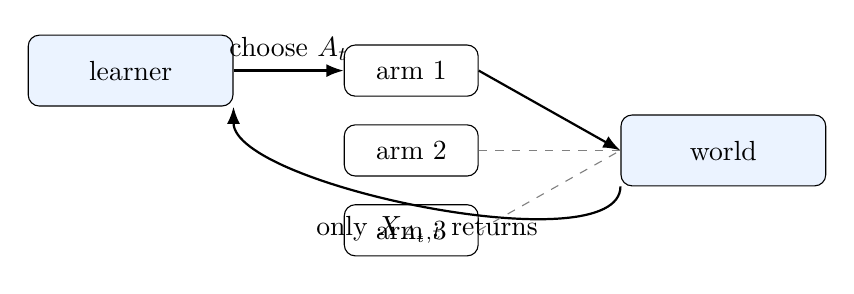
\begin{tikzpicture}[
  node distance=1.1cm,
  block/.style={draw,rounded corners,minimum width=2.6cm,minimum height=0.9cm,align=center,fill=softblue},
  small/.style={draw,rounded corners,minimum width=1.7cm,minimum height=0.65cm,align=center,fill=white},
  arrow/.style={-{Latex[length=2.2mm]},thick}
]
\node[block] (learner) {learner};
\node[small,right=1.4cm of learner] (a1) {arm 1};
\node[small,below=0.35cm of a1] (a2) {arm 2};
\node[small,below=0.35cm of a2] (a3) {arm 3};
\node[block,right=1.8cm of a2] (world) {world};
\draw[arrow] (learner.east) -- node[above]{choose $A_t$} (a1.west);
\draw[arrow] (a1.east) -- (world.west);
\draw[arrow] (world.south west) .. controls +(down:1.0cm) and +(down:1.0cm) .. node[below]{only $X_{A_t,t}$ returns} (learner.south east);
\draw[dashed,gray] (a2.east) -- (world.west);
\draw[dashed,gray] (a3.east) -- (world.west);
\end{tikzpicture}
\end{center}

The dashed arrows are the counterfactual rewards.  They exist in our mathematical imagination, but they are not observed by the learner.

\section{Regret as one-line bookkeeping}

Suppose the learner chooses arms
\[
A_1,A_2,\ldots,A_T.
\]
The oracle, who knows the best arm, receives expected reward
\[
T\mu_\star.
\]
The learner receives expected reward
\[
\E\left[\sum_{t=1}^T X_{A_t,t}\right].
\]
So the expected regret is
\[
R_T
=
T\mu_\star
-
\E\left[\sum_{t=1}^T X_{A_t,t}\right].
\]

Now write it in the useful form.  The reward of the chosen arm has conditional mean $\mu_{A_t}$.  Therefore
\[
\begin{aligned}
R_T
&=
T\mu_\star
-
\E\left[\sum_{t=1}^T X_{A_t,t}\right] \\[0.3em]
&=
\E\left[\sum_{t=1}^T \mu_\star\right]
-
\E\left[\sum_{t=1}^T X_{A_t,t}\right] \\[0.3em]
&=
\E\left[\sum_{t=1}^T \bigl(\mu_\star-X_{A_t,t}\bigr)\right] \\[0.3em]
&=
\sum_{t=1}^T
\E\left[\mu_\star-X_{A_t,t}\right].
\end{aligned}
\]
The only probabilistic step is the next one:
\[
\E[X_{A_t,t}\mid A_t]=\mu_{A_t}.
\]
Hence
\[
\begin{aligned}
\E\left[\mu_\star-X_{A_t,t}\right]
&=
\E\left[
\E\left[\mu_\star-X_{A_t,t}\mid A_t\right]
\right] \\[0.3em]
&=
\E\left[
\mu_\star-\E[X_{A_t,t}\mid A_t]
\right] \\[0.3em]
&=
\E\left[\mu_\star-\mu_{A_t}\right].
\end{aligned}
\]
Therefore
\[
\boxed{
R_T=
\E\left[\sum_{t=1}^T(\mu_\star-\mu_{A_t})\right].
}
\]

This is the basic accounting formula.  Define the gap of arm $a$ by
\[
\Delta_a=\mu_\star-\mu_a.
\]
If arm $a$ is pulled $N_a(T)$ times, then
\[
\begin{aligned}
R_T
&=
\E\left[\sum_{t=1}^T \Delta_{A_t}\right] \\[0.3em]
&=
\E\left[\sum_{t=1}^T\sum_{a=1}^K \Delta_a\ind\{A_t=a\}\right] \\[0.3em]
&=
\sum_{a=1}^K
\Delta_a\,
\E\left[\sum_{t=1}^T \ind\{A_t=a\}\right] \\[0.3em]
&=
\boxed{
\sum_{a=1}^K \Delta_a\,\E[N_a(T)].
}
\end{aligned}
\]

\begin{think}
This formula is the first real language of bandit theory.  To control regret, we do not need to predict every reward.  We need to control how often the algorithm pulls arms with positive gap.
\end{think}

\chapter{Exploration and exploitation are not slogans}

People often describe bandits by saying ``exploration versus exploitation.''  The phrase is correct, but too vague.  Regret makes it precise.

If we pull a bad arm, we lose reward now.  That is exploration cost.

If we avoid an uncertain arm too early, we may never learn that it is good.  That is exploitation cost caused by premature certainty.

The real question is:
\[
\text{How many times should uncertainty be allowed to buy more information?}
\]

\section{The two costs in one toy calculation}

Consider two arms with
\[
\mu_1<\mu_2,\qquad \Delta=\mu_2-\mu_1>0.
\]
A simple strategy is \emph{explore-then-commit}:

\begin{enumerate}
\item Pull each arm $m$ times.
\item Compare their sample means.
\item Use the arm with larger sample mean for the remaining $T-2m$ rounds.
\end{enumerate}

If the algorithm explores arm 1 exactly $m$ times, that part alone costs
\[
m\Delta.
\]
The more dangerous event is choosing arm 1 after exploration.  Let
\[
\widehat{\mu}_{1,m}
=
\frac1m\sum_{i=1}^m X_{1,i},
\qquad
\widehat{\mu}_{2,m}
=
\frac1m\sum_{i=1}^m X_{2,i}.
\]
The algorithm commits to the wrong arm when
\[
\widehat{\mu}_{1,m}\ge \widehat{\mu}_{2,m}.
\]
Since $\mu_2-\mu_1=\Delta$, this event implies at least one of the following two things:
\[
\widehat{\mu}_{1,m}-\mu_1\ge \frac{\Delta}{2},
\qquad
\mu_2-\widehat{\mu}_{2,m}\ge \frac{\Delta}{2}.
\]
Indeed, if neither happened, then
\[
\widehat{\mu}_{1,m}
<
\mu_1+\frac{\Delta}{2}
=
\frac{\mu_1+\mu_2}{2}
=
\mu_2-\frac{\Delta}{2}
<
\widehat{\mu}_{2,m},
\]
so the wrong commitment would be impossible.

Therefore, by the union bound,
\[
\begin{aligned}
\Prob(\widehat{\mu}_{1,m}\ge \widehat{\mu}_{2,m})
&\le
\Prob\left(\widehat{\mu}_{1,m}-\mu_1\ge \frac{\Delta}{2}\right)
+
\Prob\left(\mu_2-\widehat{\mu}_{2,m}\ge \frac{\Delta}{2}\right).
\end{aligned}
\]
For rewards in $[0,1]$, Hoeffding's inequality says
\[
\Prob(\widehat{\mu}_{a,m}-\mu_a\ge \varepsilon)
\le
\exp(-2m\varepsilon^2).
\]
Use $\varepsilon=\Delta/2$:
\[
\begin{aligned}
\Prob(\widehat{\mu}_{1,m}\ge \widehat{\mu}_{2,m})
&\le
\exp\left(-2m\frac{\Delta^2}{4}\right)
+
\exp\left(-2m\frac{\Delta^2}{4}\right) \\[0.3em]
&=
2\exp\left(-\frac{m\Delta^2}{2}\right).
\end{aligned}
\]
Hence the expected regret of explore-then-commit is bounded by
\[
\boxed{
R_T
\le
m\Delta
+
(T-2m)\Delta
\cdot
2\exp\left(-\frac{m\Delta^2}{2}\right).
}
\]

This is the tradeoff in its simplest form:
\[
\text{explore more} \Longrightarrow m\Delta \text{ grows},
\]
but
\[
\text{explore more} \Longrightarrow
2e^{-m\Delta^2/2} \text{ shrinks}.
\]

\begin{idea}
Exploration is not curiosity.  It is an insurance premium against choosing the wrong arm for a long time.
\end{idea}

\chapter{The algorithms in a small experiment}

We now run a small experiment.  The environment has three Bernoulli arms:
\[
(0.30,0.35,0.42).
\]
The horizon is $T=2000$, and we repeat the experiment over $500$ independent runs.

We compare four algorithms.

\section{Greedy}

Greedy uses the current sample mean and always chooses the arm that looks best:
\[
A_t\in \argmax_a \widehat{\mu}_a(t).
\]
It is natural, but fragile.  A lucky first click can make a bad arm look good.  Once that happens, greedy may keep feeding the same mistaken belief.

\section{\texorpdfstring{$\varepsilon$}{epsilon}-greedy}

$\varepsilon$-greedy mostly behaves greedily, but sometimes chooses a random arm:
\[
A_t=
\begin{cases}
\text{a uniformly random arm}, & \text{with probability }\varepsilon,\\
\argmax_a \widehat{\mu}_a(t), & \text{with probability }1-\varepsilon.
\end{cases}
\]
This is the simplest repair.  It forces the algorithm to keep looking around.

\section{UCB}

UCB chooses the arm with the largest upper confidence index:
\[
A_t\in
\argmax_a
\left\{
\widehat{\mu}_a(t)
+
\sqrt{\frac{2\log t}{N_a(t)}}
\right\}.
\]
The first term is what we have seen.  The second term is how uncertain we still are.  An arm can be chosen either because it has performed well or because it has not been tested enough.

\section{Thompson sampling}

For Bernoulli rewards, Thompson sampling keeps a Beta posterior for each arm:
\[
\theta_a\sim \mathrm{Beta}(\alpha_a,\beta_a).
\]
At each round it samples one possible world from the posterior and acts greedily in that sampled world:
\[
A_t\in\argmax_a \theta_a.
\]
A click updates
\[
\alpha_a\leftarrow \alpha_a+1,
\]
and a non-click updates
\[
\beta_a\leftarrow \beta_a+1.
\]

\section{The code that creates the comparison}

The important part is the action rule.  The environment is intentionally small, so that the algorithmic difference is not hidden behind engineering.

\begin{codeblock}[title={Core action rules for the experiment.}]{Python}
if policy == "Greedy":
    means = sums / np.maximum(counts, 1)
    a = int(np.argmax(means))

elif policy == "Epsilon-greedy":
    if rng.random() < epsilon:
        a = int(rng.integers(K))
    else:
        means = sums / np.maximum(counts, 1)
        a = int(np.argmax(means))

elif policy == "UCB":
    means = sums / counts
    bonus = np.sqrt(2.0 * np.log(max(t + 1, 2)) / counts)
    a = int(np.argmax(means + bonus))

elif policy == "Thompson sampling":
    theta = rng.beta(alpha, beta)
    a = int(np.argmax(theta))
\end{codeblock}

\section{What the experiment says}

\begin{table}[H]
\centering
\caption{Results over 500 runs, horizon $T=2000$.}
\begin{tabular}{lrrrr}
\toprule
Algorithm & Final regret & Arm 1 pulls & Arm 2 pulls & Arm 3 pulls\\
\midrule
Greedy & 137.51 & 932.35 & 366.19 & 701.46\\
$\varepsilon$-greedy & 39.85 & 140.61 & 328.29 & 1531.10\\
UCB & 67.29 & 286.26 & 470.60 & 1243.14\\
Thompson sampling & 27.77 & 98.75 & 227.37 & 1673.88\\
\bottomrule
\end{tabular}
\end{table}

\begin{figure}[H]
\centering

\includegraphics[width=0.86\linewidth]{assets/regret-exploration/regret_curves.pdf}
\caption{Mean cumulative regret.  The bands show approximately two standard errors.}
\end{figure}

\begin{figure}[H]
\centering

\includegraphics[width=0.82\linewidth]{assets/regret-exploration/pull_counts.pdf}
\caption{Mean number of pulls of each arm.  The best arm has mean $0.42$.}
\end{figure}

The greedy algorithm is not bad because it is stupid.  It is bad because it has no mechanism for doubting its early evidence.

UCB and Thompson sampling are different ways of putting doubt into the action rule.  UCB adds an explicit error bar.  Thompson sampling randomizes according to posterior uncertainty.  Both are saying: an arm that has not been tested enough should not be declared dead too quickly.

\chapter{A little probability, used as a ruler}

The probability needed for this note is modest.  We use it as a ruler for sample averages.

If arm $a$ has mean $\mu_a$, then after $n$ pulls its sample mean is
\[
\widehat{\mu}_{a,n}
=
\frac1n\sum_{i=1}^n X_{a,i}.
\]
This is a noisy ruler.  It points near $\mu_a$, but not exactly at $\mu_a$.

Hoeffding's inequality says that for rewards in $[0,1]$,
\[
\Prob\left(
\left|\widehat{\mu}_{a,n}-\mu_a\right|\ge r
\right)
\le
2\exp(-2nr^2).
\]
If we want the error probability to be at most $\delta$, solve
\[
2\exp(-2nr^2)=\delta.
\]
Step by step:
\[
\begin{aligned}
2\exp(-2nr^2)&=\delta,\\
\exp(-2nr^2)&=\frac{\delta}{2},\\
-2nr^2&=\log\frac{\delta}{2},\\
2nr^2&=\log\frac{2}{\delta},\\
r^2&=\frac{\log(2/\delta)}{2n},\\
r&=\sqrt{\frac{\log(2/\delta)}{2n}}.
\end{aligned}
\]
Thus a natural error bar is
\[
\boxed{
\widehat{\mu}_{a,n}
\pm
\sqrt{\frac{\log(2/\delta)}{2n}}.
}
\]

\begin{think}
A confidence interval is not a magical theorem.  It is just a ruler with a warning label: after $n$ samples, the ruler is wrong by more than $r$ with probability at most $\delta$.
\end{think}

\section{Why the logarithm appears}

If we check one arm once, a small failure probability is enough.  But a bandit algorithm checks many arms at many times.  We want all of the rulers to be correct at once.

Suppose there are $K$ arms and $T$ rounds.  There are at most $KT$ pairs $(a,n)$ to worry about.  If each pair fails with probability at most $2/T^4$, then the probability that any pair fails is at most
\[
KT\cdot \frac{2}{T^4}
=
\frac{2K}{T^3}.
\]
This is the union bound.  It says:
\[
\Prob(\text{at least one bad event})
\le
\sum \Prob(\text{each bad event}).
\]
Now choose the radius
\[
r_{a,n}
=
\sqrt{\frac{2\log T}{n}}.
\]
Then
\[
\begin{aligned}
\Prob\left(
\left|\widehat{\mu}_{a,n}-\mu_a\right|
\ge
\sqrt{\frac{2\log T}{n}}
\right)
&\le
2\exp\left(
-2n\cdot \frac{2\log T}{n}
\right)\\
&=
2\exp(-4\log T)\\
&=
\frac{2}{T^4}.
\end{aligned}
\]
So with high probability, for every arm and every sample size,
\[
\left|\widehat{\mu}_{a,n}-\mu_a\right|
\le
\sqrt{\frac{2\log T}{n}}.
\]

This is the mathematical reason for the UCB bonus.

\chapter{UCB proof, slowly}

We now prove the standard idea behind UCB regret.  The proof is not long.  The hard part is knowing what each line is trying to say.

Let
\[
\mathrm{rad}_{a}(t)
=
\sqrt{\frac{2\log T}{N_a(t)}}.
\]
UCB uses the index
\[
\mathrm{UCB}_a(t)
=
\widehat{\mu}_a(t)+\mathrm{rad}_a(t).
\]
At time $t$, it chooses an arm with largest index.

\section{The good event}

Define the good event
\[
\mathcal{G}
=
\left\{
\forall a,\forall n\le T:
\left|\widehat{\mu}_{a,n}-\mu_a\right|
\le
\sqrt{\frac{2\log T}{n}}
\right\}.
\]
From the previous calculation,
\[
\Prob(\mathcal{G}^c)\le \frac{2K}{T^3}.
\]

On $\mathcal{G}$, every empirical mean is close to its truth at every time.  So the rest of the proof is deterministic bookkeeping.

\section{What must be true if UCB pulls a bad arm}

Fix a suboptimal arm $a$, so
\[
\Delta_a=\mu_\star-\mu_a>0.
\]
Suppose UCB pulls arm $a$ at some time $t$.  Since UCB chooses the largest index,
\[
\widehat{\mu}_a(t)+\mathrm{rad}_a(t)
\ge
\widehat{\mu}_\star(t)+\mathrm{rad}_\star(t).
\]
On the good event,
\[
\widehat{\mu}_\star(t)+\mathrm{rad}_\star(t)
\ge
\mu_\star.
\]
Therefore,
\[
\widehat{\mu}_a(t)+\mathrm{rad}_a(t)
\ge
\mu_\star.
\]
Again on the good event,
\[
\widehat{\mu}_a(t)
\le
\mu_a+\mathrm{rad}_a(t).
\]
Combine the two inequalities:
\[
\begin{aligned}
\mu_\star
&\le
\widehat{\mu}_a(t)+\mathrm{rad}_a(t)\\
&\le
\mu_a+\mathrm{rad}_a(t)+\mathrm{rad}_a(t)\\
&=
\mu_a+2\mathrm{rad}_a(t).
\end{aligned}
\]
Thus
\[
\Delta_a
=
\mu_\star-\mu_a
\le
2\mathrm{rad}_a(t).
\]
Substitute the radius:
\[
\Delta_a
\le
2\sqrt{\frac{2\log T}{N_a(t)}}.
\]
Square both sides:
\[
\Delta_a^2
\le
4\cdot \frac{2\log T}{N_a(t)}
=
\frac{8\log T}{N_a(t)}.
\]
Rearrange:
\[
N_a(t)
\le
\frac{8\log T}{\Delta_a^2}.
\]

\begin{idea}
This is the whole UCB proof in one sentence: once a bad arm has been pulled enough, its uncertainty bonus becomes too small to hide its gap.
\end{idea}

\section{Turning pull count into regret}

If arm $a$ is suboptimal, then on the good event it can be pulled at most about
\[
\frac{8\log T}{\Delta_a^2}
\]
times.  Each pull costs $\Delta_a$.  Therefore its regret contribution is at most
\[
\Delta_a\cdot \frac{8\log T}{\Delta_a^2}
=
\frac{8\log T}{\Delta_a}.
\]
Summing over suboptimal arms,
\[
\boxed{
R_T
\lesssim
\sum_{a:\Delta_a>0}
\frac{8\log T}{\Delta_a}.
}
\]
This is called a gap-dependent bound.  It is strong when the gaps are not too small.

\section{Why small gaps are different}

If $\Delta_a$ is tiny, pulling arm $a$ is not very harmful.  The previous bound becomes large because it tries to identify a tiny difference very accurately.  But a tiny difference does not need to be identified quickly, because its regret cost is small.

A simple split captures this.  Choose a threshold $\varepsilon>0$.

For arms with small gap $\Delta_a\le \varepsilon$, the regret is at most
\[
T\varepsilon.
\]
For arms with larger gap $\Delta_a>\varepsilon$, use the UCB count:
\[
\sum_{\Delta_a>\varepsilon}
\frac{8\log T}{\Delta_a}
\le
\sum_{\Delta_a>\varepsilon}
\frac{8\log T}{\varepsilon}
\le
\frac{8K\log T}{\varepsilon}.
\]
Thus
\[
R_T
\lesssim
T\varepsilon+\frac{8K\log T}{\varepsilon}.
\]
Balance the two terms:
\[
T\varepsilon
=
\frac{8K\log T}{\varepsilon}.
\]
Then
\[
\varepsilon^2
=
\frac{8K\log T}{T},
\qquad
\varepsilon
=
\sqrt{\frac{8K\log T}{T}}.
\]
Substitute back:
\[
R_T
\lesssim
\sqrt{KT\log T}.
\]
This is a gap-independent statement.  It says that even if the gaps are tiny, regret grows much slower than $T$.

\chapter{Thompson sampling as probability matching}

UCB says: use an optimistic upper bound.  Thompson sampling says: sample a possible world and act as if that world were true.

For Bernoulli rewards, start with
\[
\theta_a\sim \mathrm{Beta}(1,1).
\]
After $S_a$ successes and $F_a$ failures,
\[
\theta_a\mid \text{data}
\sim
\mathrm{Beta}(1+S_a,1+F_a).
\]
At each round:
\[
\theta_1,\ldots,\theta_K
\text{ are sampled independently from their posteriors,}
\]
and the learner chooses
\[
A_t\in\argmax_a \theta_a.
\]

\begin{think}
Thompson sampling does not add a bonus.  It lets uncertainty itself randomize the decision.  An uncertain arm still has a chance to look best in a plausible sampled world.
\end{think}

This is why Thompson sampling often feels less mechanical than UCB.  It does not ask each arm for an explicit optimism certificate.  It asks the posterior: how often is this arm the winner in worlds that still look plausible?

In symbols,
\[
\Prob(A_t=a\mid \mathcal{H}_{t-1})
=
\Prob\left(
\theta_a=\max_j\theta_j
\mid \mathcal{H}_{t-1}
\right),
\]
where $\mathcal{H}_{t-1}$ is the data observed before round $t$.

This is sometimes called probability matching.  The probability of choosing an arm is matched to the posterior probability that the arm is optimal.

\chapter{What this language buys us}

The point of this note is not that UCB and Thompson sampling are the only algorithms worth knowing.  The point is that they teach the basic grammar of sequential learning.

\begin{center}
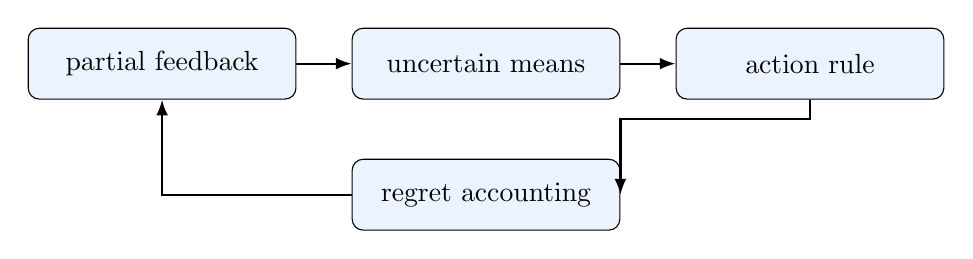
\begin{tikzpicture}[
  box/.style={draw,rounded corners,align=center,minimum width=3.4cm,minimum height=0.9cm,fill=softblue},
  arrow/.style={-{Latex[length=2mm]},thick}
]
\node[box] (feedback) {partial feedback};
\node[box,right=0.7cm of feedback] (uncertainty) {uncertain means};
\node[box,right=0.7cm of uncertainty] (rule) {action rule};
\node[box,below=0.75cm of uncertainty] (regret) {regret accounting};
\draw[arrow] (feedback) -- (uncertainty);
\draw[arrow] (uncertainty) -- (rule);
\draw[arrow] (rule.south) -- ++(0,-0.25) -| (regret.east);
\draw[arrow] (regret.west) -| (feedback.south);
\end{tikzpicture}
\end{center}

Once you see this grammar, many later topics become less mysterious:

\begin{itemize}
\item Linear bandits replace arm means by a parameterized reward model.
\item Contextual bandits let the best action depend on observed context.
\item Bayesian optimization uses posterior uncertainty over functions.
\item Best-arm identification changes the objective from earning reward to finding the best arm.
\item Reinforcement learning adds state, delayed reward, and credit assignment.
\end{itemize}

The same question keeps returning: what should an algorithm do with uncertainty when every experiment has a cost?

\chapter*{Appendix A. Symbol Table}
\addcontentsline{toc}{chapter}{Appendix A. Symbol Table}

\begin{table}[H]
\centering
\begin{tabular}{ll}
\toprule
Symbol & Meaning\\
\midrule
$K$ & number of arms\\
$T$ & time horizon\\
$A_t$ & action chosen at round $t$\\
$X_{a,t}$ & reward of arm $a$ at round $t$\\
$\mu_a$ & mean reward of arm $a$\\
$\mu_\star$ & best mean reward\\
$\Delta_a$ & gap $\mu_\star-\mu_a$\\
$N_a(T)$ & number of pulls of arm $a$ up to time $T$\\
$\widehat{\mu}_{a,n}$ & sample mean of arm $a$ after $n$ pulls\\
$R_T$ & expected cumulative regret\\
$\mathcal{G}$ & good event where all empirical means stay in their confidence bands\\
\bottomrule
\end{tabular}
\end{table}

\chapter*{Appendix B. Full Experiment Script}
\addcontentsline{toc}{chapter}{Appendix B. Full Experiment Script}

\lstinputlisting[style=blogcode,language=Python,caption={Full experiment script.}]{assets/regret-exploration/regret-exploration-simulation.py}

\backmatter
\nocite{lattimore2020bandit,bubeck2012,auer2002,russo2018,srinivas2010gpucb}
\printbibliography[heading=bibintoc,title={References}]

\end{document}
